\documentclass[11pt]{article}
\usepackage{fullpage}
\usepackage{graphicx}
\usepackage{natbib}
\usepackage{hyperref}
\usepackage{enumitem}

\begin{document}
\title{Digital Lab: Sampling, Fourier Transforms, Mixers, and Down-Converters}

\maketitle

    The purpose of this lab is to experimentally investigate digital
sampling, digital Fourier transforms, and mixers. Mixers are the basis
of heterodyne spectroscopy. Heterodyne spectroscopy, in turn, is what
you use every day that you listen to a radio, use a cell phone, or watch
TV---or do radio astronomy.  

Most heterodyne applications use the more common double-sideband (DSB)
mixer, for which the upper and lower sidebands produce identical mixer
output. Here we also explore single-sideband (SSB) mixers, which display
the remarkable property that upper and lower sidebands produce outputs
at negative and positive baseband frequencies, respectively. In real
life, SSB mixers allow such things as the transmission and reception of
stereo FM signals; in olden days, FM transmission were all monophonic.
Later in the course, we will use an SSB mixer for our first measurements
of the 21-cm line of interstellar atomic hydrogen (HI). 

In his lab, you will be performing several experiments, analyzing the
data and generating a number of different data files. You will need to
keep careful notes in your {\bf lab notebook}! Or, pay the penalty, and
forget what you did, do things twice, and be completely
disorganized. Your choice!

\paragraph{Goals:}
\begin{itemize}[noitemsep,nolistsep]
\item Learn how to sample electronic signals---here, one or more sine
  waves---digitally using our computers.
\item Become acquainted with the basic law of sampling: the Nyquist
  criterion.
\item Learn how to use Digital Fourier Transforms (or Discrete Fourier
  Transform; DFT) to determine the
  frequency spectrum of a signal.
\item Learn about the Fast Fourier Transform (FFT) as a particular, and
  particularly fast, implementation of the DFT.
\item Learn the basics of mixing for frequency conversion (that's
  the {\it heterodyne} technique) and for measuring phase.
\item Construct a two-output mixer, composed of two mixers, that can be
  operated as either a DSB or an SSB mixer.
\item Use the two-output mixer in DSB and SSB modes and understand the
  difference.
\item Learn how complex inputs to a FT break the negative/positive
  frequency degeneracy.
\item Develop proficiency in Python, using it for the
  mathematical analysis, signal processing, and making nice plots.
\item Continue to improve the quality of your Latex write up and graphs.
\end{itemize}

\paragraph{Schedule:}

As before, there's a lot to do in this lab! If you don't understand the Nyquist criterion
by the end of the first week, you're behind. Here's how it should be:

\begin{enumerate}[noitemsep,nolistsep]
% XXX check references
\item Finish \S \ref{nyquist},
  \S \ref{pwrspectrum}, \S \ref{leakage} below. Be prepared to show your
  results to the class, making real-time plots in Python.
\item Finish \S \ref{upperlowerdsb} and \S \ref{digital_mixing}
  below. Again, be prepared to show your results to the class.
\item Finish \S \ref{fir_filter} and \S \ref{ddc}
    Write your formal report!
  It should follow the standard format, consisting of an introduction,
  discussion of experimental activities and results, description of the
  analysis technique, presentation of analysis results, and
  discussion/interpretation. With all this, you should hand in a
  reasonable number of plots together with commentary to illustrate your
  work, your thought processes, and your conclusions.
\end{enumerate}

\section{Week 1: Sampling and Analog Mixing}
\label{sec:week1}
\subsection*{Prerequisites}

\begin{itemize}[noitemsep,nolistsep]
\item Discrete Fourier Transform
\item Convolution Theorem
\item Nyquist Sampling
\end{itemize}

\subsection*{Materials}

\begin{itemize}[noitemsep,nolistsep]
\item 2 local oscillators
\item digitizer (either ROACH or Pulsar sampler card)
\end{itemize}

\subsection{Command and Conquer: Running the System from the Command Line}\label{software}

    This lab will require lots of adjustments and measurements to be made,
over and over and over\footnote{You get my point here...} again. This can be
rather painful to have to do by hand, but thanks to software you don't have
to! In particular, you are going to need to control two different types of
devices: the SRS Function Generators (sometimes called local oscillators or
`LOs') and the Pulsar sampler. To control either of these devices from the
command line, you will need to import the Digital Front-End Control (DFEC)
module into your instance of python. Within this module are two functions: 
\verb set_srs  and \verb sampler .

    The \verb set_srs  function is used to control the two LOs that exist in
the lab, creatively labeled \emph{SRS1} and \emph{SRS2}. With these LOs, you
can control the frequency (which must be between $0 < \nu \le 30
\textrm{ MHz}$), the power (in either dBm or $V_{pp}$, set so that the output
voltage does not exceed $\pm 5$ Volts) and the phase (which
must be between $0^o \le \phi < 7200^o$.) In order to set the LOs, use the
following:
\begin{verbatim}
In [1]: import DFEC
In [2]: srsNumber = 1
In [3]: DFEC.set_srs(srsNumber,freq=1e6,off=0,dbm=0,off=0,pha=0)
\end{verbatim}
The only required input for the function is the first value, which corresponds
to the name of the LO being controlled (1 for SRS1 and 2 for SRS2 -- this
value should be an integer!). The above command will set SRS1 to 1 MHz, 
with the power set to 0 dBm (i.e. 1 mW), with a 0 Volt DC offset and a phase
offset of 0 degrees. The arguments/inputs for
for \verb freq  , \verb vpp , \verb dbm \footnote{The function will error out
if you try to set both the power by specifying both the dBm and the $V_{pp}$,
since they both control the same thing.}, \verb off , and \verb pha  are all
optional, such that if you do not specify values for these things, the
software will leave the LOs with whatever settings they last had. In practice,
it is a good idea to specify any arguments whose setting you are not sure off,
like when someone other than yourself had changed to settings on the LO last.

    The \verb sampler  function is used to control the sampler on Pulsar (the
small computer sitting next to the rack). Pulsar has two main modes for
operating -- single and dual channel. When you use the sampler, you should
make sure that your BNC cables are connected to the appropriate location: the
single channel connector is on the far right of the row of inputs, the dual
channel are the left and middle connectors. To get data from the sampler, use
the following command:

\begin{verbatim}
In [4]: nSamp = 1000
In [5]: sampFreq = 1e7
In [5]: data = DFEC.sampler(nSamp,sampFreq,fileName='mydata.txt',dual=True)
\end{verbatim}
The two required inputs for the function are the number of samples to record
(must be between 1 and 262144) and the sampling frequency (must be less than
20 MHz for single channel mode, 10 MHz for dual channel mode). The above
command will sample data in dual channel mode, writing the data to disk in a
file called \verb mydata.txt , recording 1000 values at a sampling rate of 10
MHz, and returning (in python) the values recorded as an array of values,
which are recorded as variable \verb data .
\\
\\
\noindent\emph{Documentation for both functions exist, so when in doubt, read the manual!}

\subsection{Nyquist Sampling and Aliasing: A Single Sine Wave} \label{nyquist}

    Here we explore the all-important realms of the Nyquist
criterion and aliasing in digital sampling.  Clearly, if you sample too
slowly the signal won't be well-reproduced.  But if you sample really
fast, then you generate large data files that take a long time to
process.  Just how slowly can you sample the signal without completely
losing its basic properties (such as, for example, the fact that it
oscillates with frequency $\nu_{sig}$)?

The fundamental parameter here is the ratio of sampling frequency
$\nu_{smpl}$ to signal frequency $\nu_{sig}$. With our equipment we can set
$\nu_{smpl}$ to only selected, quantized values. However, we can set
$\nu_{sig}$ with almost arbitrarily high precision. So to explore these
issues we will pick a sampling frequency $\nu_{smpl}$ and take data at
several signal frequencies $\nu_{sig}$.  Be sure to use a coax T so that
you can look at the sampled signal on the oscilloscope.  Set the
peak-to-peak voltage appropriately so that it doesn't saturate the
Analog-to-Digital Converter (known as the ADC).

\subsubsection{Your First Digital Sampling}
    We want to explore sampling rate issues, so to that end
we will begin by\dots
\begin{enumerate}[noitemsep,nolistsep]
\item Pick a convenient sampling frequency $\nu_{smpl}$.  
\item Set the synthesizer to frequency $\nu_{sig} = (0.1, 0.2,
      0.3, \dots, 0.9) \nu_{smpl}$ and take data. 
\end{enumerate}

\noindent Take $N$ contiguous samples with $N$ an integral power of 2, say
$N=256$.  Throughout the data-taking, you should always be
monitoring the signal with the oscilloscope. These are sine waves, so
it's easy to measure the period by looking at the oscilloscope; each
time you digitally sample the signal, you should write down the period
(maybe in your lab notebook?).  

For each dataset, plot the digitally sampled waveform versus
time.  In particular, make the digital plot informative, meaning that
you can clearly see the signal shape; if necessary, plot only a part of
the data so you can clearly see the signal shape (e.g., a few cycles of
the sine wave); compare this with the oscilloscope trace.  Also, for all
the datasets derive and plot the Fourier power spectrum.  Make sure that
you {\it label the axes} with proper values of time and frequency---and
choose convenient units, such as microsec and megaHz, to avoid huge and
tiny numbers.  In deriving the Fourier spectra, use our homegrown DFT
procedure (see \S \ref{pwrspectrum} below).

Now, look at both sets of these plots and note any funny business.
Think about your results and draw your own conclusion: just what is the
minimum sampling rate that you can get away with? (That's Nyquist's
  criterion). 

\subsubsection{Let's Go to Extremes\dots}

By now you might have an idea of what's going on. Test yourself:
try the following two experiments. But before analyzing the
results, predict to yourself what they will look like. How? Use
good old-fashioned paper and pencil to make some diagrams. If you can
successfully predict the following, then you really understand
the Nyquist criterion! So here we go:

\begin{enumerate}[nolistsep,noitemsep]
\item Repeat the above for $\nu_{sig} = \nu_{smpl}$. 
\item Now make $\nu_{sig} \over \nu_{smpl}$ really large!
        In other words, blatantly violate Nyquist's criterion!
        Our oscillators won't run faster than 30 MHz, so to
        accomplish this you'll have to use not only a large
        $\nu_{sig}$ but also change $\nu_{smpl}$ to be very
        slow. Use as large as a ratio as you can, but make sure that
        the ratio is not an integral or half-integral number. Take lots of
        samples. Look at the sampled waveform.  What do you get?
        Why?
\end{enumerate}

\subsection{For your Lab Report}

\noindent In your report, select a well-considered set of plots to
illustrate what you've learned, and compose a well-written commentary
that convinces me that you really understand what's going on. Also
clearly state what you have concluded regarding Nyquist's criterion. 

    With your plots, you can save paper by fitting multiple plots on a page
by using Pylab's \verb$subplot$ function.

\subsection{Using FFT's to Calculate a Power Spectrum} 
\label{pwrspectrum}
 
\subsubsection{The Analytic Fourier Transform}

        The input to the Fourier transform is voltage versus time, say
$E(t)$; the output is voltage versus frequency, say $E(\nu)$.  The Fourier
transform is the integral
 
\begin{equation} \label{ift}
E(\nu) = {1 \over T} \int_{-T/2}^{T/2} E(t) e^{2 \pi j \nu t} dt \ .
\end{equation}
 
\noindent The input voltage is real; it is multiplied by the complex
exponential and integrated, so the output is complex. Of particular
importance is that he Fourier Transform is invertible: you can go
from the time to the frequency domain, and from the frequency domain you can
get back to the time domain using the inverse transform

\begin{equation}
E(t) = {1 \over F} \int_{-F/2}^{F/2} E(\nu) e^{-2 \pi j \nu t} dt \ .
\end{equation}
 
\noindent Note: If you're paying attention, you would wonder how
$F$ and $T$ are defined above. In the proper analytic formulation, they
are both infinity. We emphasize their boundedness here because, in
practice, i.e.\ when you do numerical calculations, neither can be
infinity!

\subsubsection{The Discrete Fourier Transform (DFT)} \label{dft}

Our voltage versus time is not continuous, but rather it is discrete
samples. With the digital transform, the integral becomes a sum. In
this sum, you need to specify:
\begin{enumerate}[noitemsep,nolistsep]
\item The set of sample times. I strongly suggest:
\begin{enumerate}[noitemsep,nolistsep]
\item  Using $N$ samples, where $N$ is even (and even better: a power of 2).
\item Use the center
  channel as the zero point. With $N$ even, there is no center channel,
  so make the times run from ${-N \over 2}/
  \nu_{smpl}$ to $({N \over 2} -1)/ \nu_{smpl}$.
\end{enumerate}
% XXX does below need to be adapted to python?
\item The output is a function of frequency, so you have to specify the
  frequencies for which you want the output $E(\nu)$. I strongly
  suggest that, at first, you calculate the the output for $N$
  frequencies running from $-{\nu_{smpl} \over 2}$ to $+{\nu_{smpl}
  \over 2} \left( 1 - {2 \over N} \right)$. This makes the frequency
  increment equal to  $\Delta \nu = \nu_{smpl}/N$. Thus, you
  calculate a voltage spectrum running from $-{\nu_{smpl} \over
  2}$ to about ${\nu_{smpl} \over 2}$ using our in-house DFT procedure.

Later on, if you are intellectually daring and curious, try doubling or
tripling the frequency range, keeping the separation $\Delta \nu$ the
same (i.e., by increasing the number of output frequencies to $2N$ or $3N$).

\end{enumerate}

\begin{equation}
P(\nu) = E(\nu) E(\nu)^* \ .
\end{equation}
 
\noindent In Python, there are two ways to get this product.  One is to use
the \verb$numpy.conj$ function, i.e.\ {\tt PF = EF * np.conj(EF)}.  Should the
imaginary part of \verb$PF$ be zero? (answer: yes! Why is this?) Is it?
(answer: no! Why not?) To get rid of this annoying and extraneous
imaginary part, you can use the \verb$float$ function: 
\verb$PF = PF.astype(np.float)$. 
 
The other (more convenient and suggested) way is to square the 
complex vector, i.e.\ \verb$PF = np.abs(EF)**2$. The result is
automatically real.

\subsubsection{OPTIONAL: The Fast Fourier Transform (FFT)} \label{fft}
% XXX I think this shouldn't be optional

Above in \S \ref{dft}, you had $N$ time samples and evaluated the DFT
for $N$ well-chosen frequencies. These were ``well-chosen'' because for
these particular values of frequency---and only these particular
values---you can get back to the time domain by using the inverse
transform.

It so happens that, for these particular combinations of frequency and
time, there is a very fast algorithmic implementation called the 
  Fast Fourier Transform, the FFT. What do we mean by ``Fast''? Well,
normally when you do a DFT, you have $N$ input numbers and $N$ output
numbers and the number of calculations $\propto N^2$. When $N$ gets large,
this takes a long time to calculate! For the FFT, on the contrary, the
number of calculations $\propto N {\rm ln}_2(N)$, and this makes it
possible to do large-$N$ transforms. 

If you have the time and energy, try Numpy's FFT and compare it to
your DFT calculation above. The FFT output is ordered in what you might
think is a funny and awkward way; however, it's really not awkward
for most applications. See our ``DFT's with DFT's'' handout for details.

\subsection{ Leakage Power and Frequency Resolution} \label{leakage}

\subsubsection{Leakage Power}

Above, you calculated a power spectrum for each input signal at $N$
distinct frequencies separated by $\Delta \nu = \nu_{smpl}/N$. In each,
you found a spike corresponding to the input signal's frequency. Here,
focus on just one of the properly-sampled signals $\nu_{sig}$. Calculate
the power spectrum for many more than $N$ output frequencies over the
Nyquist range $\left[-{\nu_{smpl} \over 2} \ {\rm to}\ +{\nu_{smpl}
\over 2} \left( 1 - {2 \over N} \right)\right]$; i.e., make the
frequency increment much smaller than $\Delta \nu = \nu_{smpl}/N$.
Making the output frequencies closer together gives a more nearly
continuous frequency coverage in the plot of the output spectrum.  Turn
up the vertical scale a lot to see if there is any nonzero power at
frequencies other than $\nu_{sig}$.  You do see such power! This
is Spectral Leakage. It affects all power spectra calculated using
Fourier techniques. 

Can you understand what's going on from a mathematical viewpoint?

\subsubsection{Frequency Resolution}

If you had two sharp spectral lines, how closely spaced in frequency
could they be and still resolve them? Roughly, this is just the apparent
width of the line when plotted against frequency. Look at the width of
the line for your plot of \S \ref{leakage} above. Compare this width to
$1 \over T$, where $T$ is the total time span over which the samples
were taken. If you have the inclination, try taking other time series
with varying number of samples (and thus, varying $T$) and confirm any
relationship between line width (that is, frequency resolution) and
$T$.

Can you understand this from a mathematical viewpoint?

\section{Week 2}
\subsection*{Prerequisites}

\begin{itemize}[noitemsep,nolistsep]
\item Heterodyne Mixers
\item Data Representations
\item Digital Down Conversion
\end{itemize}

\subsection*{Materials}

\begin{itemize}[noitemsep,nolistsep]
\item 3 local oscillators
\item digitizer (both ROACH and Pulsar sampler card)
\end{itemize}

\subsection*{Some Thoughts}

This week we will mix some sine waves together to observe their beat frequencies.  We will first do this
in analog to learn a bit about heterodyne mixing, but then we will migrate the mixing part into a powerful
digital processor, setting up the work next week, where we will control a down-conversion signal
chain implemented entirely on this digital processor.

\subsection*{FPGAs and Simulink}

We're just getting started on our digital part of the class, and we haven't really had a chance to talk
about Field Programmable Gate Arrays (FPGAs) or how they are programmed --- that's going to come next
week.  However, we're going to use one today, so let's cover what you need to know.

\subsubsection*{The ROACH}

The Reconfigurable Open Architecture for Computing Hardware (ROACH) is an open-source board (e.g.
all schematics, board design, etc. are free and open) developed by the CASPER collaboration, which
was started here at Berkeley (by Dan Werthimer and Aaron Parsons) and is now pan-global.  
On this board is a Virtex-5 FPGA made by Xilinx, along with a CPU.  The CPU
runs linux (you can ssh into it), using a special linux kernel cooked up by CASPER that allows it to support 
automatic interfaces to some of the logic you program the FPGA with.

FPGAs are programmed with ``bit files'' that you load onto the chip, and tell the circuitry inside what
wires to connect to what logic components.  To load a bit file onto the ROACH FPGA, you execute a *.bof file
from the CPU (relevant BOF files are in the \verb+lab_digital/misc+ directory of the Git repository for
the class).  The BOF file contains both a bit file, as well as some other information that allows
linux to interface to the FPGA.  After running a BOF file (leave it running), you need to find the 
process ID of that program.  The linux command ``jobs'' should do the trick.

If you try to run a BOF file and receive a ``Resource Busy'' error, that means another BOF file is
already running on the FPGA (FPGAs can't have multiple personalities simultaneously).  That BOF file
must be killed before a new one can be run.

\begin{figure}\centering
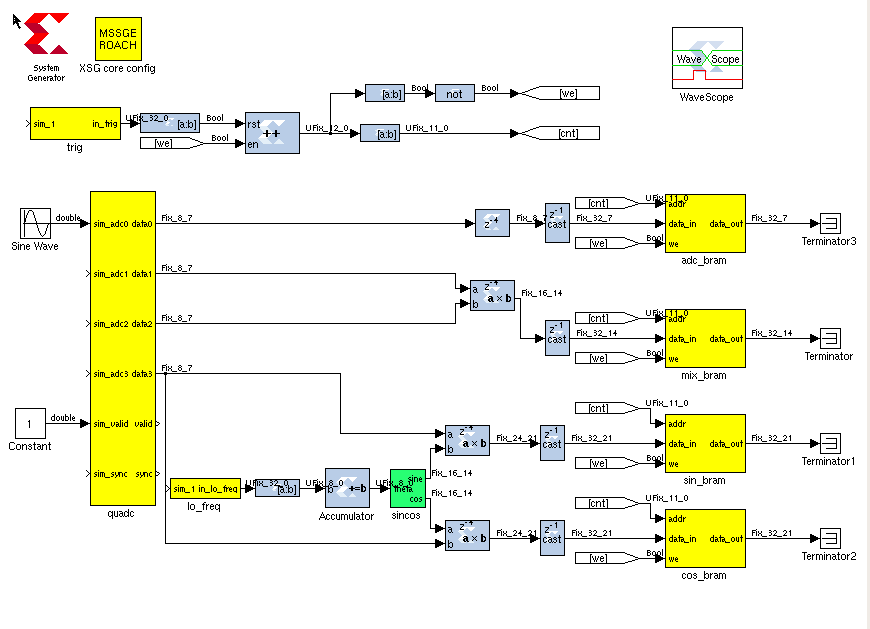
\includegraphics[width=6in]{plots/adc_snaps.png}
\caption{
The sampler design (in the Simulink programming language) that was compiled into the 
``adc\_snaps'' BOF file used in Week 2.  Yellow blocks represent interfaces between
the FPGA and the outside world.  The block ``quadc'' interfaces to the ADC card that
is plugged into the ROACH;  ``trig'' and ``lo\_freq'' are software registers that
appear as one-word (8 byte) files on the ROACH when the BOF file is executed, and
``adc\_bram'', ``mix\_bram'', ``sin\_bram'', and ``cos\_bram'' are memories that
appear as larger files holding samples.  White pentagons (pointing left and right) are
named signals that connect to any other pentagon with the same name.  For example
``we'' stands for ``write enable'' and connects to every BRAM, as well as feeding
back into the same counter that generates ``we''.  Other white blocks (``Terminator'',
``Sine Wave'', ``Constant'') are for simulation only, and do not affect the compiled circuit.
} \label{fig:adc_snaps}
\end{figure}

Finally, if you go to a secret directory /proc/PID/hw/ioreg (where PID is the process ID), you'll find
a bunch of files that have names that correspond to some of the blocks in the schematic diagram in Figure \ref{fig:adc_snaps}.
The schematic above is an actual FPGA program.  It tells the FPGA to read samples from an interface to
the quad-ADC (described below), and place them into a BRAM (block random access memory) until it is full.
The address to which samples are written is supplied by a counter that stops itself at the final address
of the BRAM, and waits for a signal to come in over the register ``trig'' to reset the counter back to
0 and allow it to write new samples in into the memory.  You'll notice that ``trig'' and ``data\_bram''
are files in the ioreg directory; those are your interfaces to the register that triggers a data capture,
and the data itself that is written into the BRAM.  You can write a value to the file ``trig'', and you can
read values out of the file ``data\_bram'', just as if they actually were files.  But they are not.  They
are interfaces to the FPGA.  But Python doesn't know that.

So all you need to know now is this: that ``trig'' is an unsigned 32-bit integer (Ufix\_32\_0, in
Figure \ref{fig:adc_snaps}), and the least-significant bit
controls the counter reset button.  The BRAM holds signed 32-bit samples for each ADC sample.  The
ADC is natively an 8-bit sampler, and its sample clock is controlled by a function generator feeding the
SMA port marked ``clk''.  Happy sampling.  Note, the QuadADC card that is connected to the ROACH introduces
a {\bf small DC (0 Hz) offset to the signals it samples.  You'll definitely see this when you start
analyzing and Fourier transforming signals in this lab, and you'll need to identify and explain these features
for your lab report}.


\subsection{Basic Double Sideband (DSB) Mixer Operation: Upper and Lower Sidebands}
\label{upperlowerdsb}

        For this, use two SRS synthesizer oscillators as inputs to a
mixer to explore the spectra and waveforms in the DSB mixing process.
The SRS synthesizers work up to 30 MHz.  Assign one of the SRS
synthesizers to be your ``local oscillator'' (LO) with frequency
$\nu_{lo}$, and the other your ``signal'' with frequencies $\nu_{sig} =
\nu_{lo} \pm \delta \nu$.  Here, you choose the frequency difference
$\delta \nu$ and you set the two synthesizers, one to the lo
frequency and the other to the signal frequency. There are two cases for
the signal frequency, $\nu_{sig} = \nu_{lo} + \delta \nu$ and
$\nu_{sig} = \nu_{lo} - \delta \nu$.  Make $\delta \nu$ somewhat small
compared to $\nu_{lo}$, maybe $5\%$ of $\nu_{lo}$.  For the input power
level, a good choice is 0 dbm\footnote{What does this ``dbm'' mean? It's
the power relative to 1 milliwatt, expressed in decibels (dB). For our
system the cable impedance is 50 ohms; what's the rms voltage for a
signal with power level 0 dBm?} for both synthesizers.

        We will want to digitally sample the mixer output and explore
both the sum and difference frequencies. As you learned in the Fourier
lab, there are extremely important issues regarding sampling rate. The
most basic is the Nyquist criterion. For this lab, we also want enough
samples per period to give you a reasonable facsimile of the sine wave
when you plot it; from this standpoint, it's not unreasonable to sample
at twice Nyquist, or even faster.  Another issue is the number of
points you sample, which must be large enough to give you at least a
few periods of the slowest sine wave.

        From what you know about mixers, what is the fastest sine wave
in the output? This, combined with our above comment and the upper limit
on our sampling frequency (20 MHz for single channel, 10 MHz for dual
channel), would determine the upper limit on $\nu_{lo}$.

\subsubsection{The Mixer}

Combine the two signals, $\nu_{lo}$ and $\nu_{sig}$, in a mixer for the
two values of $\nu_{sig}$.  For the mixer use a Mini-Circuits
ZAD-1, which has three BNC connectors (three {\it ports}) and works well
at these frequencies.  The ZAD-1, like nearly all mixers, has its ports
labeled ``R'' (the ``RF'' or ``signal''); ``L'' (the ``local
oscillator''); and ``X'' (the ``mixing product'') or ``I'' (the
``intermediate frequency'').  However, as we explain below, these labels
are misnomers.  They are based on the usual use for a mixer, which is to
take two high frequency signals as the inputs to the R and L ports and
produce a low frequency difference frequency as the output at the I
port.

        The ZAD-1 is a balanced mixer, so the ``R'' and ``L'' ports are
identical, and in particular will not couple to DC or very low
frequencies.  In contrast, the ``I'' port is coupled differently and
will handle voltages all the way down to, and including, DC.  The mixing
process functions no matter which two ports are used as inputs.  For
example, if you are using a mixer to modulate a high frequency (say, a
few MHz) with a low frequency (say, a few kHz), you should use the ``I''
port for the low frequency and either of the other two for the high
frequency; take the output from the third port.

We will want to look at the output, which consists of both the sum
and difference frequencies, so choose the ports appropriately. Digitally
sample the mixer output for both cases ($\nu_{sig} = \nu_{lo} \pm \delta
\nu$).

\subsubsection{For Your Lab Report} \label{digsamp}

        For the two cases, plot the power spectra versus
frequency. Explain why the plots look the way they do. In your
explanation include the terms ``upper sideband'' and ``lower sideband''.

For one of the cases, plot the waveform.  Does it look like the
oscilloscope trace? Also, take the Fourier transform (not the power
spectrum) of the waveform and remove the sum frequency component by
zeroing both the real and imaginary portions (this is ``Fourier
filtering'').  Recreate the signal from the filtered transform by taking
the inverse transform; see \S \ref{fourierfilter} to see how this is
done. Plot the filtered signal versus time.  Explain what you see.

\subsubsection {On  Fourier Filtering} \label{fourierfilter}

When you use DFT to go from the time to the frequency domain, you
specify the times and the sampled voltages as input and calculate the
output for a well-chosen set of frequencies.  These times and
frequencies should be symmetric around zero, as we strongly suggested above in \S
\ref{pwrspectrum}.  To filter out the high-frequency mixed signal, you
have to zero both the real and imaginary high-frequency components,
and you must zero both the negative and positive frequencies. In
frequency space, these zeroed values must be symmetric.

To go back from the frequency domain to the time domain, use the 
  filtered frequency Fourier components (which are complex) and their associated frequencies
  as inputs and calculate the output for the original times.
  You should also use {\tt numpy.ifft}, which keeps the
  amplitude scale correct (check the documentation in IPython).
  The output will be a time series, and because you've
  eliminated the sum frequency component, the only thing that remains
  should be the difference frequency component.

One more thing. The output of the inverse transform had better be
real---after all, your original input was real! You'd better check this!
If it isn't real, then either (1) you didn't treat the negative and positive
frequencies symmetrically when you zeroed the signal, or (2) you didn't
use our suggested input times and output frequencies. If you're having
trouble, check your basic technique by doing the inverse transform on
the non-filtered Fourier components; you should recover the original
time samples.

\subsection{Digital Mixing (DSB and SSB) on an FPGA} \label{digital_mixing}

Now we are going to do the exact same thing as in \S\ref{upperlowerdsb}, but digitally.

First, let's make sure we can interact with the ROACH board (see ``Some Thoughts'', above)
to digitize an analog signal and read out the digital data.  In contrast to the CPU-hosted ADC
used in Week 1, this week we will need to acquire data directly from the FPGA hosted on the ROACH.
This entails:
\begin{itemize}[noitemsep,nolistsep]
\item connecting the signal to be digitized to port 1 of the ADC card (SMA 1, please keep signal amplitudes around -10 dBm)
\item connecting the sample clock to the clock port of the ADC card (SMA 3, choose an appropriate sample rate $\le200$ MHz, with
    and amplitude of 0 dBm)
\item logging onto the ROACH board (root@roach.ugastro.berkeley.edu)
\item launching the BOF file for the sampler/mixer FPGA design
\item writing the correct values to the file interface to the ``trig'' register
\item reading the binary data out of the file interface to the ``adc\_bram'' memory onto another computer
where you will do your analysis (using scp).
%\item interpreting the binary data as numbers using the correct binary format and endian-ness
%\item plotting/analyzing your data to make sure it makes sense
\end{itemize}

Once you have acquired some data, write a Python script that
interpreting the binary data as numbers using the correct binary format and endian-ness
and plots your data to make sure it makes sense; \verb+numpy.fromfile+ is a good place to start.  
So\dots convince yourself that your data
makes sense.  What is the time interval between each sample?  What is the signal amplitude
relative to full-scale for the ADC?

Once you understand your data, connect the output of your mixer from \S\ref{upperlowerdsb} to
the same ADC input and collect some more data.  Interpret the resulting waveform and decide if
it makes sense. Optionally, you might compare the samples you collect on the FPGA to those obtained from the CPU-hosted
ADC.  

Now here's the exciting part.  Ports 2 and 3 (SMA 2 and 5) on the ADC card are also digitized, but then are multiplied
post-digitization before the result is written to ``mix\_bram'' (triggering the data capture is still
done through ``trig'').  Now you can take each of the signals
that were mixed together in analog, connect them to Ports 2 and 3, and compare the digitally mixed output
to the result you obtained with an analog mixer.

Finally, instead of mixing two input signals digitally, we will mix a single signal with an LO that is
derived from the sample clock.  In this case, connect the signal that we want to mix with to Port 4 (SMA 6)
on the ADC card.  Next, before triggering to acquire your data, write a carefully chosen value
into the file interface to the ``lo\_freq'' register.  This register maps the 0 to $2\pi$ interval
of an oscillator to addresses from 0 to 255.  For each ADC sample that comes in, the number stored
in ``lo\_freq'' is added to the current address (wrapping around to 0 after 255), and the sine/cosine
evaluated at the corresponding point between 0 and $2\pi$ is output for mixing with the incoming signal.
The result, as many ADC samples come in, is that the input waveform is multiplied with sine/cosine waveform
of a frequency that is determined by ``lo\_freq''.  Choose an appropriate value to write in this register,
and be sure to record what the corresponding frequency of your digital LO is.

Now you may trigger your data capture.  The result of mixing the input signal with a cosine wave of your
chosen frequency is stored in ``cos\_bram'', while the output of mixing with a sine wave is recorded
in ``sin\_bram''.  Use the data stored in each of BRAMs to reconstruct the {\it complex valued} sinusoid
that this digital Single-SideBand (SSB) mixer outputs.  Compare this recorded waveform to what you
expect for a SSB mixer, given the frequency of the LO and the frequency of your input signal.

\subsubsection{OPTIONAL: Dealing with DC offsets}

As you have (likely) already discovered, your FPGA sampled data doesn't just have
a single tone (i.e. a signal at a single frequency), but also appears to have a DC signal as well.
What's going on? Well, the problem here is that different devices have a different reference
point for what 0 Volts means. Part of the reason for this is physical (depending on how the device
is, among other things, grounded). Part of this is slightly arbitrary -- after all, the ADC only
tells you a 8-bit value that happens to correspond to \emph{some} range in voltage that the
signal is currently within. In a perfect world, one of these levels would be perfectly centered on 0 Volts. When it doesn't, this makes things a complete mess, because that DC signal will mix with \emph{all the signals you are mixing your input with}. So, for our digital DSB mixer, you will see up to 9 tones, instead of the 3 or 4 tones that you should see. We need to get rid of these spurious tones, lest they contaminate our result!

There are two ways to accomplish our task at hand. First, we can call back to our experience in Section \S\ref{fourierfilter}. You should know what mixing products are going to be created, which means that it should be pretty easy to select those frequency bins and zero them out. Again, make sure that you treat your data symmetrically -- failing to do so will mean that your output voltage will be complex, and in the real world we deal with real values\footnote{This isn't entirely true, but nonetheless, your original output was in real Volts -- why shouldn't your new voltages be so as well?}!. Fourier transform your data back into a series of voltages in time, and plot your result. Does this method work? Could you see some potential limitations with this method?

Sometimes, the best plan to dealing with problems is not to try and fix it in the digital/computing side, but rather in the analog side. In this case, there is a DC offset between what the ADC thinks is 0 V, and what the SRS oscillator thinks is 0 V. The easiest way to fix this is to adjust the DC voltage on the SRS device (see the documentation for the \verb set_srs  function on how to do this). You can try and make some educated guesses on what these offsets are, change the offsets and rerun the experiment over and over again. Or, if you are clever, you can use the information in the Fourier transform to help guide you to what your voltage offsets are. The whole point of using a Fourier transform is to be able to translate a series of voltage measurements in time into a series of frequencies with specified voltage (in this case, measured peak to peak). If you do your math right, the output of your DFT \emph{will be} the offset voltage that exists. You should keep in mind that the sampler can measure between $\pm1$ V, and that there are a total of 256 levels (i.e. it's an 8-bit sampler). When you finish, make a plot (logarithmic might be best) of the result -- if you close enough to perfect, you should only see power at two frequencies: your LSB and USB! Why might this be better than Fourier filtering?

One additional note -- when measuring the DC output of two mixed signals (each with their own DC bias), you are going to be measuring the product of their DC bias multiplied against one another (and if the signals have the same frequency, the lower sideband of their mixing product!). If you use the DC output to help you adjust your voltage\footnote{This isn't the only way to do this...}, you should choose two different frequencies to mix together, and try adjusting only one DC offset at a time.

\subsubsection{For Your Lab Report}

        Plot the power spectra versus
frequency for the digital and analog DSB mixing cases. Explain why the plots look the way they do.  Identify
key features (including the DC offset signal from above).  For the digital mixing case, plot the waveform.

Also plot the power spectrum of the output of the digital SSB mixer.  As before, explain why the plot
looks as it does, and in particular, explain the difference between the SSB mixing case and the DSB mixing
case that you explored.  Plot the waveform (both real and imaginary components on one plot). Also, apply a
Fourier filter to extract the single tone that you are interested, and plot that on the same plot.
Determine
whether the extracted waveform has a positive or negative frequency.

In all cases, make sure that the frequency/time axes have appropriate physical units (Hz, $\mu$s, etc.).
It is not acceptable to just have these axes as sample counts.

Finally, explain some of the advantages and disadvantages of DSB and SSB mixers for both digital and
analog implementations.  In comparing digital and analog implementations of SSB mixers, consider what the effects would
be if the sine/cosine components were slightly out of phase with each other (you can simulate this to find out).  Which
case would be more likely to have such phase errors?

\section{Week 3}
\subsection*{Prerequisites}

\begin{itemize}[noitemsep,nolistsep]
\item Synchronous and Asynchronous Logic
\item Processor Architectures
\item FIR Filters
\end{itemize}

\subsection*{Materials}

\begin{itemize}[noitemsep,nolistsep]
\item 1 local oscillator
\item ROACH board
\item broad-band noise source
\item 1 analog filter
\end{itemize}

\subsubsection*{The ROACH, revisited}

\begin{figure}\centering
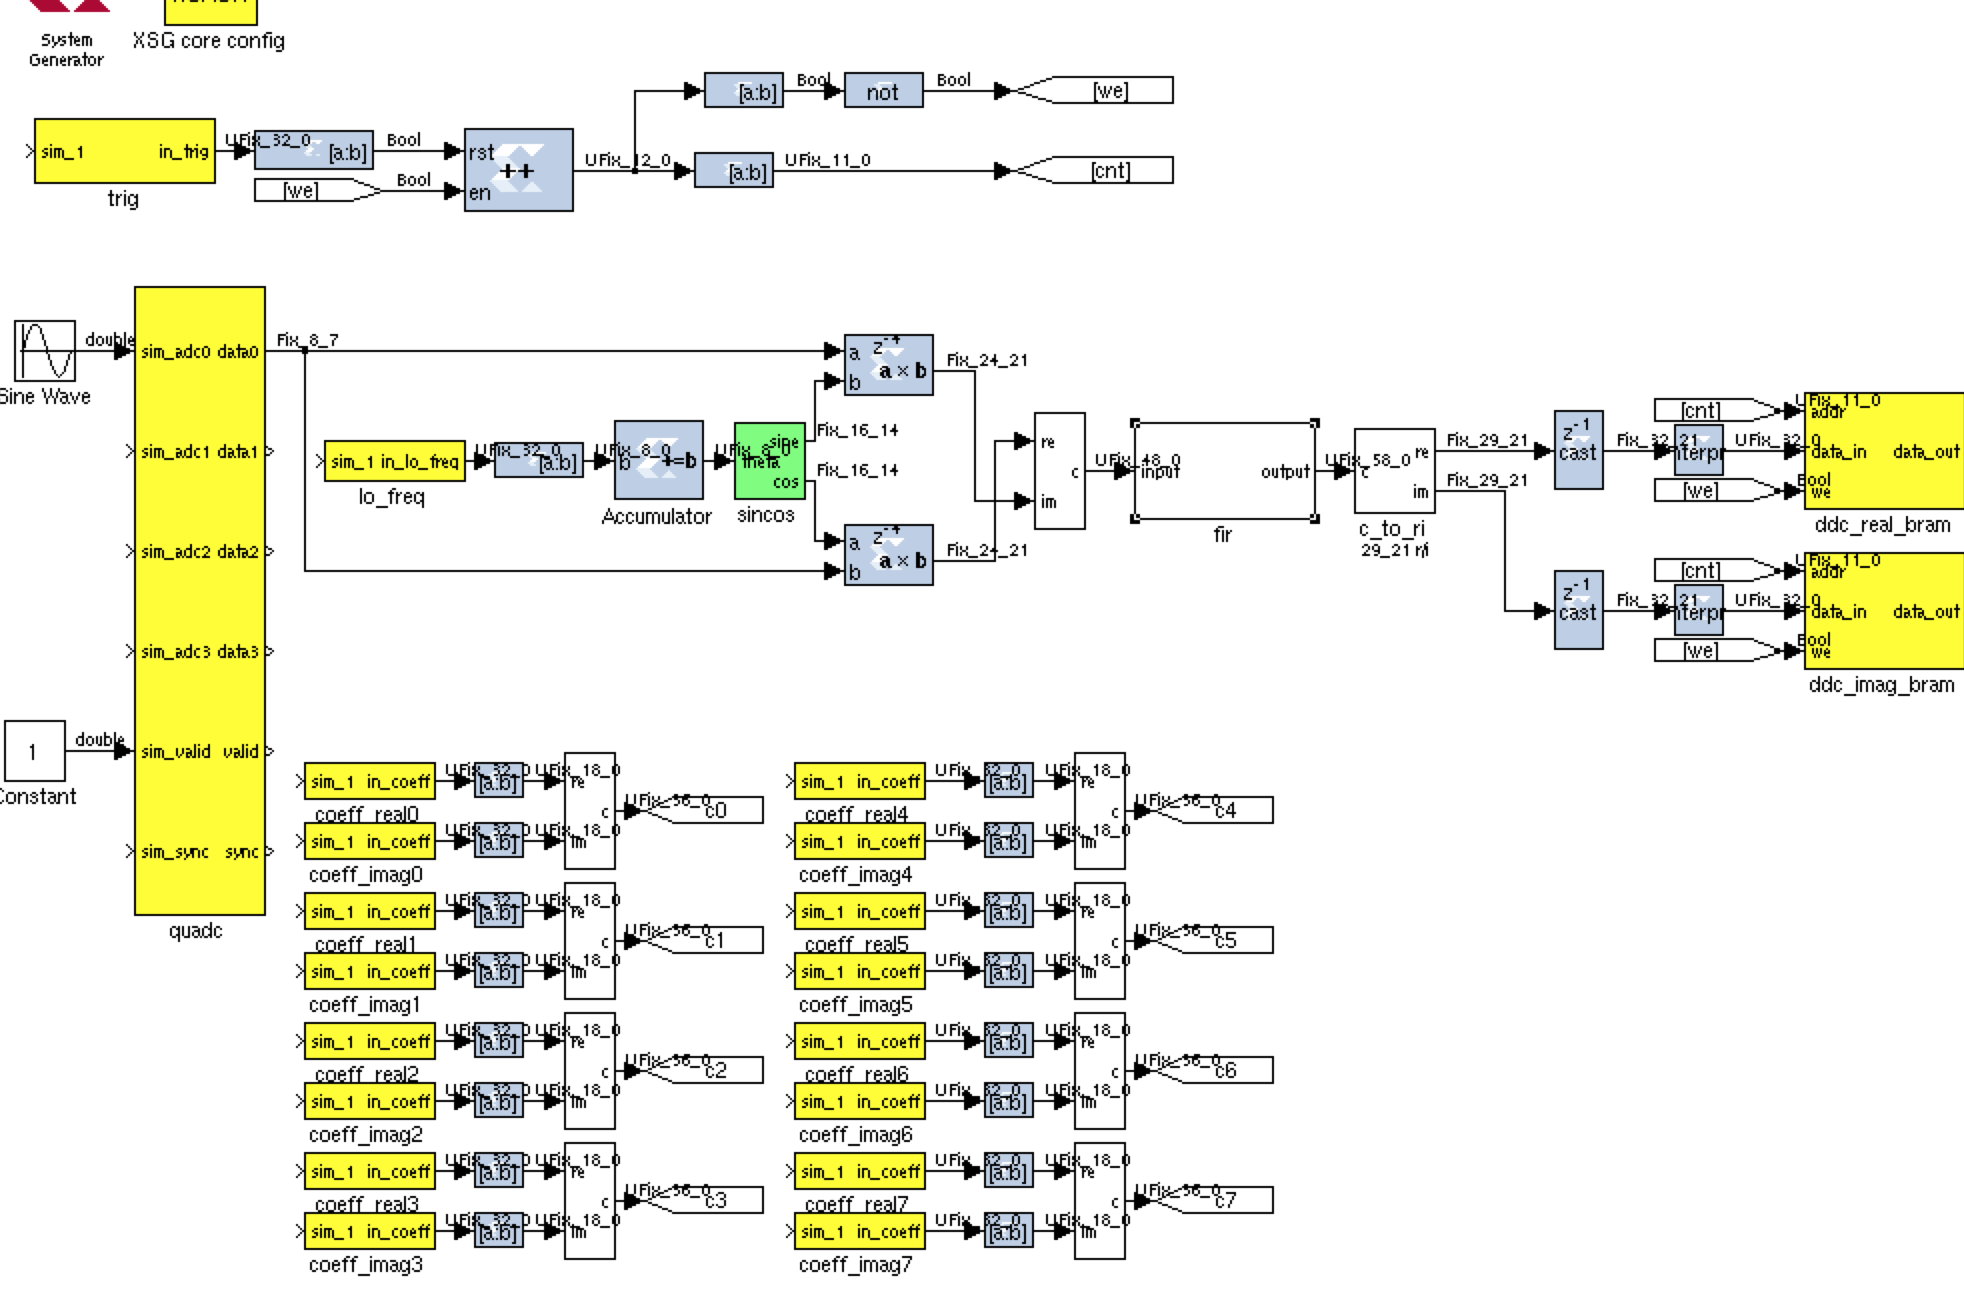
\includegraphics[width=6in]{plots/ddc_overview.png}
\caption{
The FPGA design that was compiled into the 
``dig\_dwn\_conv\_2'' BOF file used in Week 3.  This design includes a mixer with a digital
LO, which outputs complex samples to an FIR filter.  The filtered (complex) output samples
are written to the BRAMs at the right of the figure.
Many portions of this design
(trig, lo\_freq) operate similarly to the ``adc\_snaps'' design (Fig. \ref{fig:adc_snaps}).
The ``fir'' subsystem (the white block in the center-right) is expanded in
Figure \ref{fig:fir_subsystem} to show what happens inside.  Of primary importance
are the ``coeff\_real'' and ``coeff\_imag'' registers, which are used to input the desired
FIR coefficients to the FIR filter.
} \label{fig:ddc_overview}
\end{figure}

\begin{figure}\centering
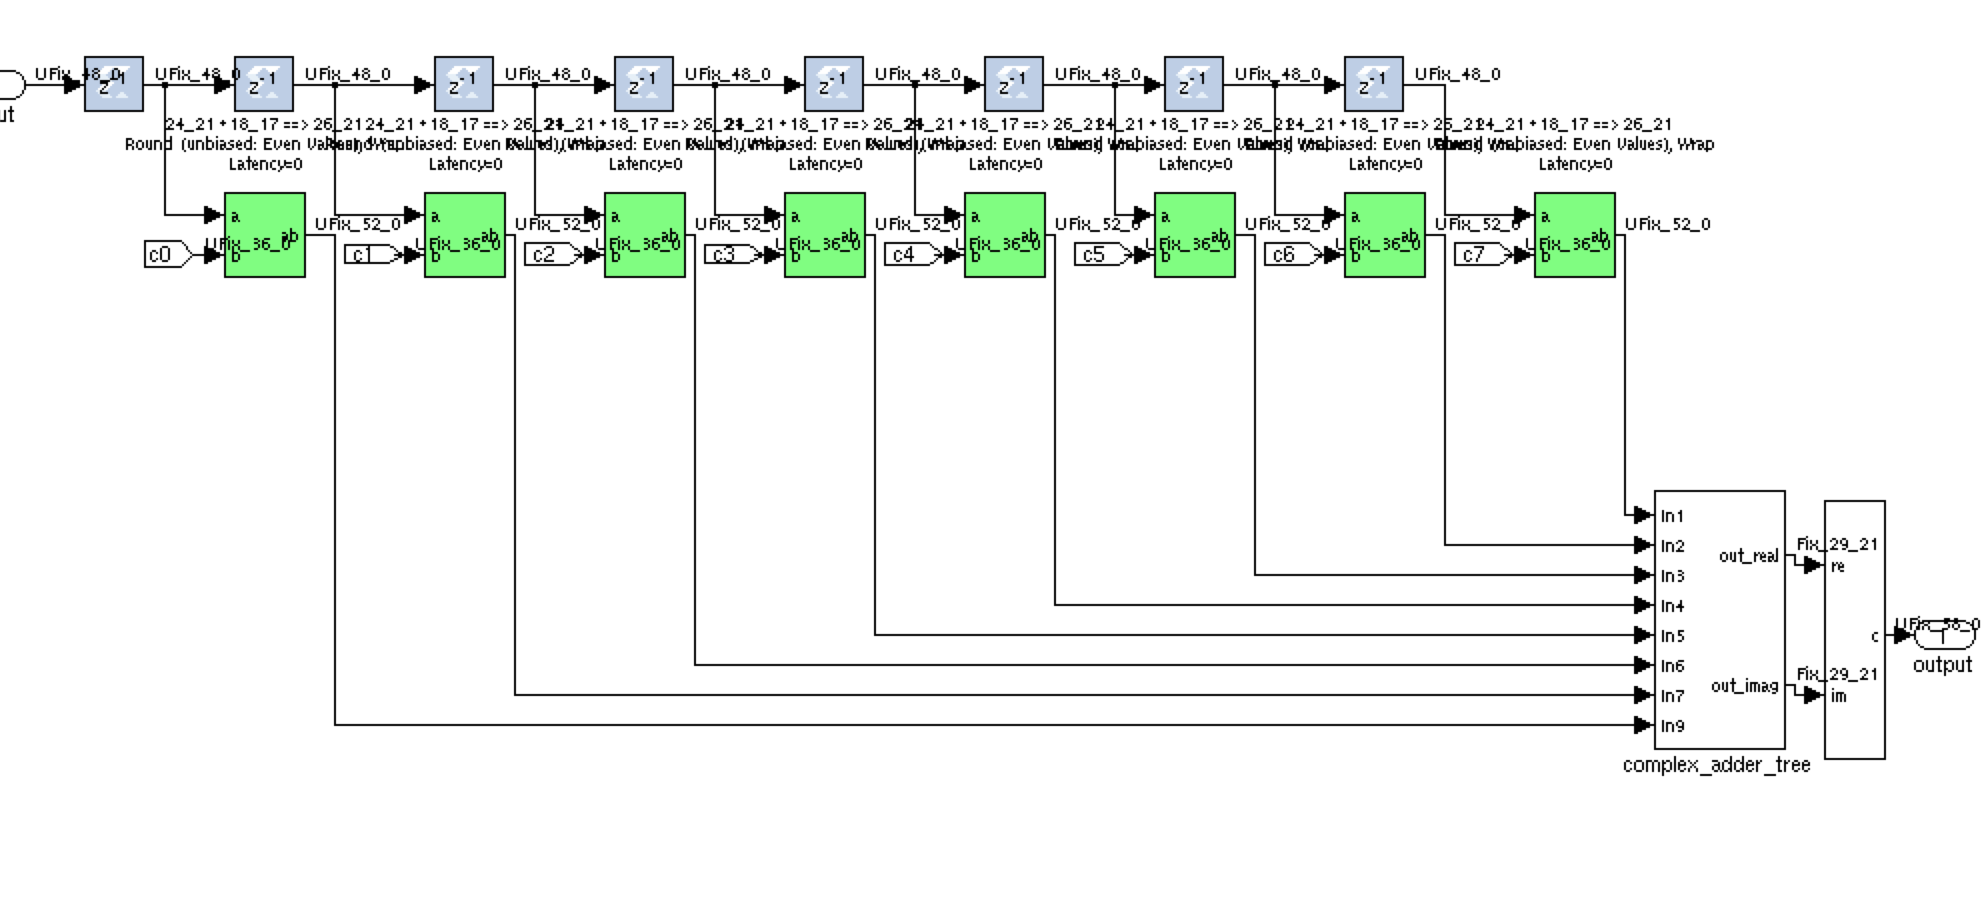
\includegraphics[width=6in]{plots/fir_subsystem.png}
\caption{
An expansion of the FIR subsystem in Figure \ref{fig:ddc_overview}.
Input samples are buffered along the top, and delayed samples are tapped 
downward into complex multiplies (green) that are also fed with coefficients.
Note the correspondence between the ``c[0-7]'' labels used here and the 
concatenated output of coefficient registers in Figure \ref{fig:ddc_overview}.
The products of all of these multipliers are summed in an adder tree
for complex values.  An example of a real-valued adder tree is shown in Figure \ref{fig:adder_tree}.
} \label{fig:fir_subsystem}
\end{figure}

\begin{figure}\centering
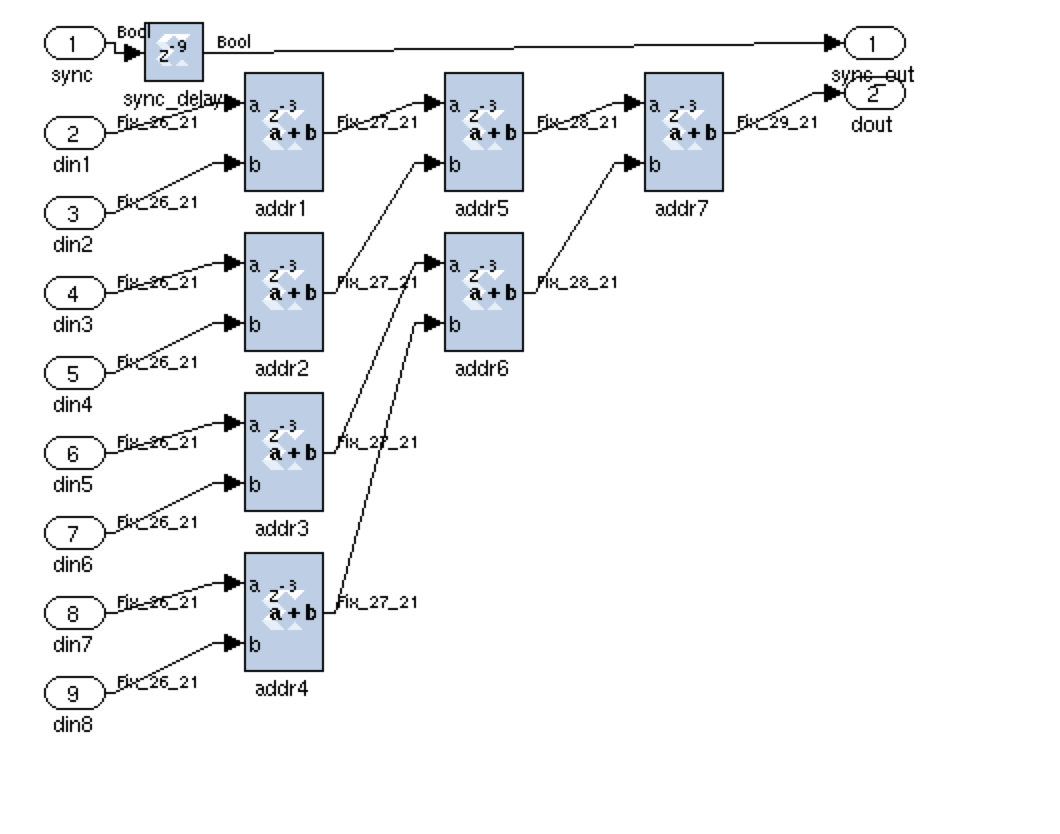
\includegraphics[height=3in]{plots/adder_tree.png}
\caption{
An illustration of a (real-valued) adder tree similar to the one used
in Figure \ref{fig:fir_subsystem}.
} \label{fig:adder_tree}
\end{figure}

From last week, you'll have a little experience running BOF files on the ROACH.  You probably
remember that, when running the BOF file, you can go to a secret directory 
/proc/PID/hw/ioreg (where PID is the process ID) to find
files correspond to registers and memories that are attached to the CPU, which are highlighted
in yellow in Figure \ref{fig:ddc_overview}.
You'll see that ``trig'' and ``lo\_freq'' behave identically to the ADC sampler design
in Figure \ref{fig:adc_snaps}, which is described in Week 2.

This week has two major differences.  The first is the addition of registers for inputting the
coefficients for the FIR filter circuit.  These registers are labeled 0 to 7 for the eight
taps of the FIR filter shown in Figure \ref{fig:fir_subsystem}.  Each coefficient is a complex
number so, for example, the 0th coefficient has two registers: ``coeff\_real0'' and ``coeff\_imag0''.
Each ``coeff'' register technically holds 32 bits, but only the lower 18 bits are connected to
the circuit.  The other bits don't matter---you can put anything in them.  But for those 18 bits,
they each represent a signed 2's complement number, with 17 digits after the binary point
(i.e. a Fixed18\_17).  In Figure \ref{fig:ddc_overview}, you'll see that these are labeled ``UFix'',
but they are actually re-interpreted as signed in the complex multipliers in Figure \ref{fig:fir_subsystem}.

In this portion of the lab, you'll need to pay attention to that binary point.  If you want your signal
to pass through strongly, you'll have to write in values that are close to 1. (But be careful! Can you
actually represent +1 with a Fix18\_17 number?)  Otherwise, the FIR filter will heavily attenuate
your signal, and you might not get anything in the output BRAMs.

\subsection{Coefficients for an FIR Filter} \label{fir_filter}

As you should have seen in lecture videos, Finite Impulse Response (FIR) filters are
able to implement frequency-domain filters with a tunable shape that is determined
by the coefficients that they convolve with an input waveform.
Also, now that you've had a bit of a preview of the capabilities of FPGAs, and how they function,
you might appreciate how their architecture makes them particularly adept at implementing
FIR filters, which have a natural pipelined flow to them.

In the first part of this section of the lab, we will choose the coefficients for an FIR filter that is running
on the ROACH as part of a larger Digital Down-Converter:
\begin{itemize}[noitemsep,nolistsep]
\item Choose coefficients that implement a 5/8-band filter (a filter that, if you divided the band into 8 
(positive/negative) frequency channels, would extract the 5 channels centered around 0):
\begin{itemize}[noitemsep,nolistsep]
\item Choose the frequency-domain response you want for your filter (i.e. the function you would like to multiply
the frequency spectrum of your noise by to ``filter" it)
\item Compute the complex, time-domain coefficients that implement that filter, keeping in mind that: 
\begin{itemize}[noitemsep,nolistsep]
\item Multiplication in the frequency domain is a convolution in the time domain
\item The Fourier transform of a real-valued signal has the property that:
$\hat f(\omega) = \hat f^*(-\omega)$
\item You will want to think carefully about where the 0 frequency bin is
\item The FFT puts negative frequencies after positive frequencies in your array.  Similarly, when you take the inverse, it will put negative times after positive times.  When implementing your coefficients in an FIR, though, negative times {\it have} to operate on samples that arrive before positive times.
\end{itemize}
\end{itemize}
\item In what order are you going to write these coefficient into the software registers of your FIR filter?
\item Plot the predicted filter response for your coefficients at a frequency resolution much finer than an 8-channel
DFT produces.  The best way to do this will be to add more time-domain samples to your coefficients.  We don't want to introduce any new signal, though, so just add zeros to pad your coefficients out to 64 samples, and then transform the result back into the time domain.  
\item Why aren't the passband and stopband flat?
\end{itemize}

\subsubsection{For Your Lab Report}

Produce a table that indicates the (floating point) coefficients you intend to
use.  Next, we'll need to convert these coefficients to fixed-point numbers
that we can write to the FPGA.  Assuming that software registers will be
interpreted on the FPGA as 18-bit signed integers with 17 bits after the binary
point, what binary values will you use to represent these coefficients?

Also, plot the desired (ideal) bandpass of your filter, along with the actual
response that (as determined above) is not quite what you ideally wanted.
Explain why this filter deviates from your ideal.  Is it possible to perfect
this filter?

\subsection{Putting it all together for a Digital Down-Converter} \label{ddc}

Now you are going to use your coefficients to program the coefficients of an FIR filter running on the
FPGA which has been chained onto the end of the digital mixer from the previous week (Fig. \ref{fig:ddc_overview}).  
You can control
the LO and the shape of a filter that follows to implement a Digital Down-Converter (DDC) that mixes and filters
an input signal according to your every whim.

What we'd like to do now is to empirically characterize the shape of the filter you have implemented.  
You can input sine waves of a fixed amplitude and different periods and use the amplitude of the recorded
waveform to determine the filter response at that frequency.  This works fine, but another (equivalent) way
that may be easier to automate is to change the frequency of your LO, which will change where the sum/difference
frequencies appear within your FIR filter function.  Do whichever is easier for you.  In either case, you'll
probably want to write a Python program that automates the process.

So set up signal input to the DDC on Port 1 of the ADC.  Program your FIR coefficients and choose an appropriate
LO frequency.  Trigger a capture.  On the BRAMs entitled ``ddc\_real\_bram'' and ``ddc\_imag\_bram''
will be the complex output signal.  Don't forget to grab data from both BRAMs and assemble the values
into a single complex number.  As you are familiar with from last week, there will be two different tones
in the output data.  Each characterize the FIR filter at a different frequency.  You may want to use
Fourier filtering to isolate each one independently for characterizing your FIR filter.

Now determine the attenuation between the input and output signal as a function of frequency.  This will
give you, empirically, the shape of your FIR filter (and its placement in the band as a result of your LO).

\subsubsection{For Your Lab Report}

Compare your empirically determined filter shape with the (non-ideal) filter shape you calculated in the previous section.
Are they the same?  If not, you should figure out why not.  This is a digital system, so you can expect exactness, down to the
level of the residual noise.

Generate a plot that overlays the filter shape you were shooting for, the filter shape you computed would actually
be generated by your 8 FIR coefficients, and your measurements of the filter shape.  Make sure this plot has
a frequency axis that is in physical (Hz) units, and that the y-axis (the power) is consistent between all 3 versions
of the plot.  To normalize the amplitude of your sine waves, it might help to know what the amplitude of
an unfiltered sine wave is.  This can be easily generated by setting all of your FIR coefficients to 0, except
for one of them, which you set to approximately 1.  Can you explain why this works, and how it can be used
to normalize your plot?

\end{document}
